\section{System Architecture}
\label{sec:architecture}

\textsc{HOOX} consists of ten specialized Workers (Table~\ref{tab:workers}) that together form a complete trading pipeline. Two additional Workers---\texttt{pine-worker} and \texttt{pyne-worker}---provide Pine Script tooling and are outside the core production mesh.

\begin{table}[t]
  \centering
  \caption{Core \textsc{HOOX} Workers. Only \texttt{hoox} and \texttt{dashboard} expose public endpoints.}
  \label{tab:workers}
  \small
  \begin{tabular*}{\linewidth}{@{\extracolsep{\fill}}llp{5.5cm}l@{}}
    \toprule
    \textbf{Worker} & \textbf{Role} & \textbf{Key responsibilities} & \textbf{Trigger} \\
    \midrule
    \texttt{hoox} & Gateway & Auth, WAF, rate limiting, idempotency & Webhook/API \\
    \texttt{trade-worker} & Execution & Multi-exchange order placement & Binding/Queue \\
    \texttt{agent-worker} & Risk manager & Trailing stops, take-profit, kill switch & Cron \texttt{*/5} \\
    \texttt{telegram-worker} & Notifications & Alerts, RAG queries, bot commands & Binding \\
    \texttt{d1-worker} & Data layer & Centralized D1 SQLite access & Binding \\
    \texttt{email-worker} & Email ingress & Mailgun webhook parsing & Webhook \\
    \texttt{web3-wallet-worker} & DeFi & On-chain swaps and contract calls & Binding \\
    \texttt{analytics-worker} & Observability & Analytics Engine time series & Binding \\
    \texttt{report-worker} & Reporting & Twice-daily PDF generation & Cron 08:00, 18:00 UTC \\
    \texttt{dashboard} & User interface & Portfolio monitoring (Next.js/OpenNext) & Public UI \\
    \bottomrule
  \end{tabular*}
\end{table}

\subsection{Architectural Overview}

Figure~\ref{fig:architecture} depicts the ingress, compute, storage, and external exchange layers. Public signals enter only through \texttt{hoox} (webhooks) or channel-specific Workers (\texttt{email-worker}, \texttt{telegram-worker}). All downstream execution uses Service Bindings; only \texttt{trade-worker} and \texttt{web3-wallet-worker} initiate outbound HTTPS to external APIs.

\begin{figure}[!htbp]
  \centering
  \IfFileExists{figures/architecture.pdf}{%
    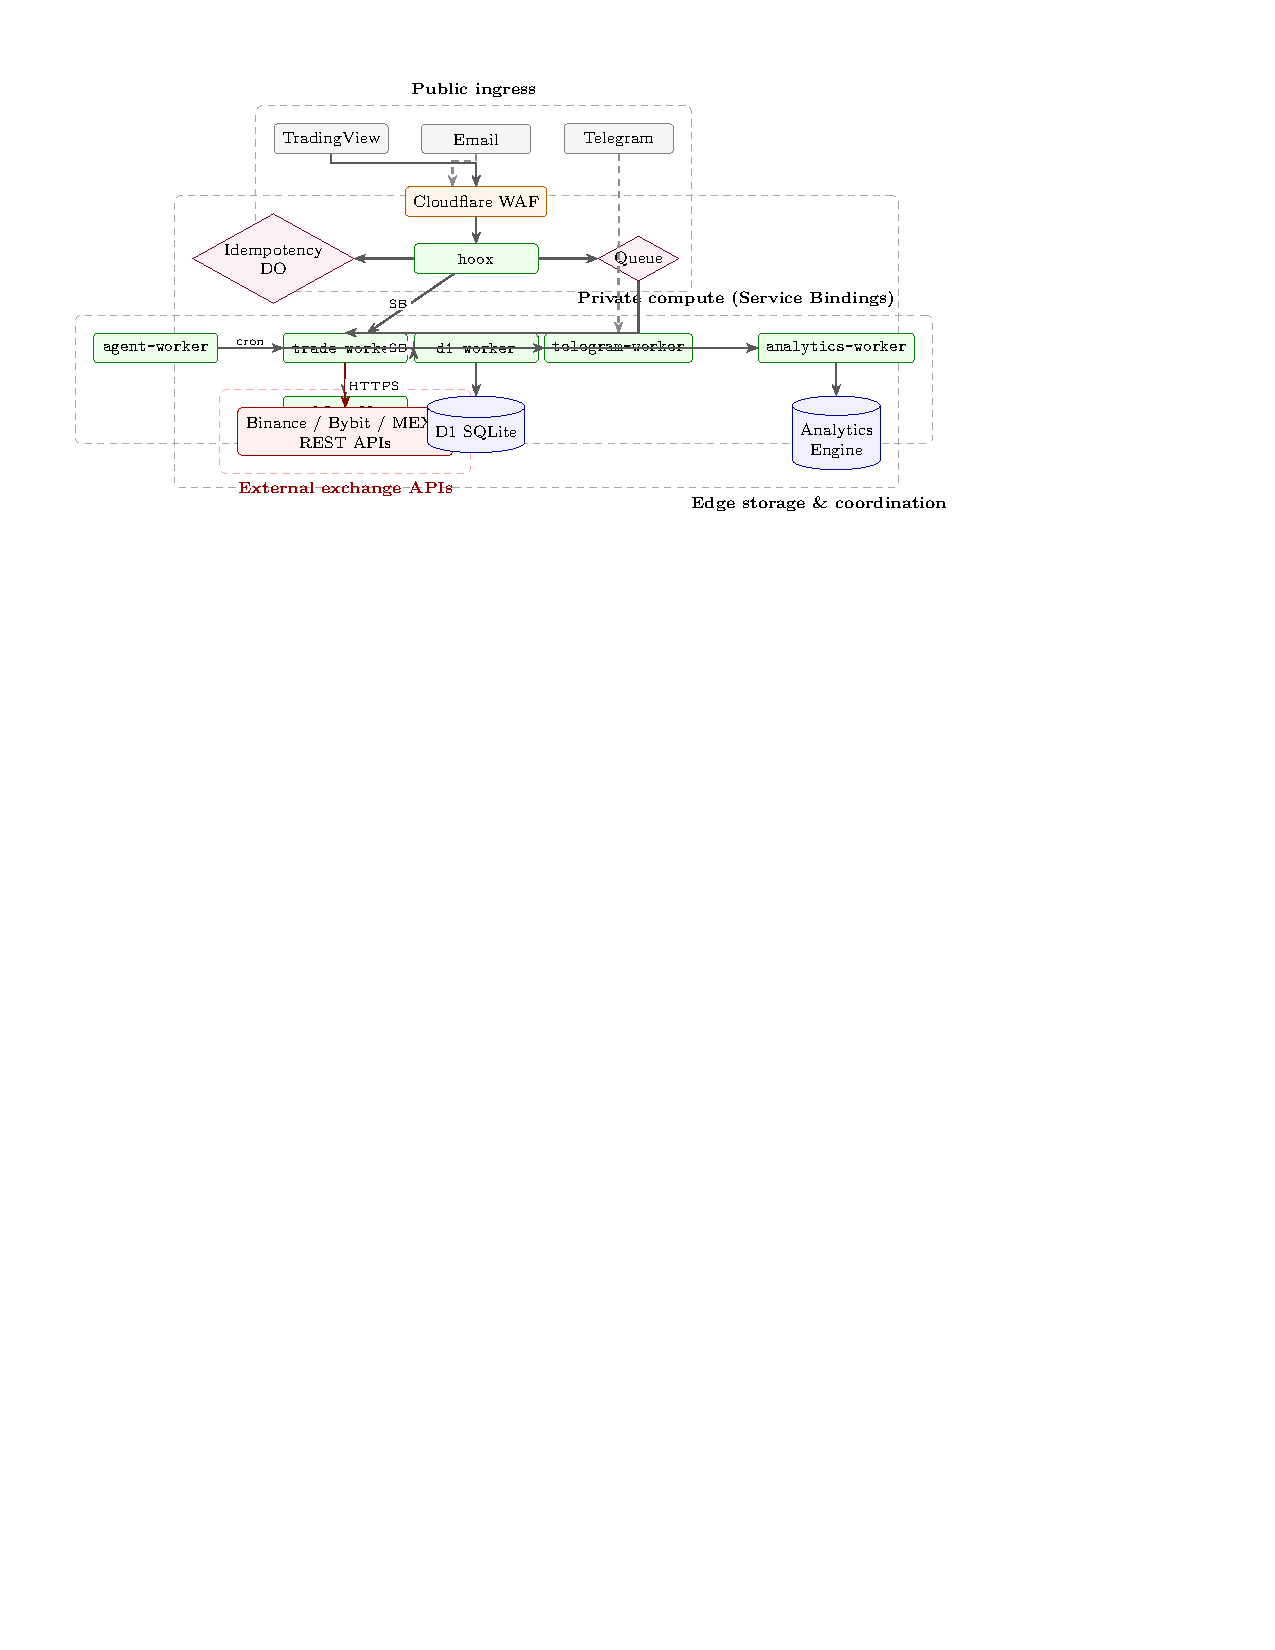
\includegraphics[width=\linewidth]{figures/architecture.pdf}%
  }{%
    \ifhooxusetikz
      \resizebox{\linewidth}{!}{% TikZ architecture diagram for HOOX (included by hoox-arxiv-paper.tex)
% Layout: 4 horizontal rows
%   row 1 (y=4.0): public ingress sources (TradingView / Email / Telegram)
%   row 2 (y=2.6): Cloudflare WAF
%   row 3 (y=1.4): hoox gateway with Idempotency DO and Queue flanking it
%   row 4 (y=-0.4): private compute mesh (5 workers, 2.6cm spacing)
%   row 5 (y=-1.8): storage + external exchange APIs
\begin{tikzpicture}[
  x=1cm, y=1cm,
  ext/.style={draw=black!50, rounded corners=2pt, fill=gray!8,
    minimum width=1.9cm, minimum height=0.55cm, font=\footnotesize, align=center, inner sep=2pt},
  waf/.style={draw=orange!70!black, rounded corners=2pt, fill=orange!8,
    minimum width=2.2cm, minimum height=0.55cm, font=\footnotesize, align=center, inner sep=2pt},
  worker/.style={draw=green!50!black, rounded corners=2pt, fill=green!8,
    minimum width=2.2cm, minimum height=0.55cm, font=\footnotesize\ttfamily, align=center, inner sep=2pt},
  store/.style={draw=blue!60!black, rounded corners=2pt, fill=blue!6,
    minimum width=1.9cm, minimum height=0.55cm, font=\footnotesize, align=center, inner sep=2pt},
  coord/.style={draw=purple!60!black, rounded corners=2pt, fill=purple!6,
    minimum width=2.0cm, minimum height=0.55cm, font=\footnotesize, align=center, inner sep=2pt},
  exchange/.style={draw=red!60!black, rounded corners=2pt, fill=red!6,
    minimum width=2.6cm, minimum height=0.55cm, font=\footnotesize, align=center, inner sep=2pt},
  layer/.style={draw=black!35, dashed, rounded corners=3pt, inner sep=0.35cm},
  layerlabel/.style={font=\scriptsize\bfseries},
  arrow/.style={-{Stealth[length=1.8mm]}, semithick, draw=black!65},
  extarrow/.style={-{Stealth[length=1.8mm]}, semithick, draw=red!55!black},
  sb/.style={font=\scriptsize, fill=white, inner sep=1pt}
]

  % ── Row 1: external ingress sources (3 sources spread horizontally) ──
  \node[ext] (tv) at ( 3.0, 4.0) {TradingView};
  \node[ext] (em) at ( 6.0, 4.0) {Email};
  \node[ext] (tg) at ( 9.0, 4.0) {Telegram};

  % ── Row 2: Cloudflare WAF (centered under sources) ──
  \node[waf] (waf) at ( 6.0, 2.6) {Cloudflare WAF};

  % ── Row 3: hoox gateway + coordination primitives ──
  \node[worker] (gw)    at ( 6.0, 1.4) {\texttt{hoox}};
  \node[coord]  (ido)   at ( 3.0, 1.4) {Idempotency\\DO};
  \node[coord]  (queue) at ( 9.0, 1.4) {Queue};

  % ── Row 4: private compute mesh (5 workers, 2.6cm spacing) ──
  \node[worker] (tw)  at ( 0.0, -0.4) {\texttt{trade-worker}};
  \node[worker] (d1w) at ( 2.6, -0.4) {\texttt{d1-worker}};
  \node[worker] (tgw) at ( 5.2, -0.4) {\texttt{telegram-worker}};
  \node[worker] (aw)  at ( 7.8, -0.4) {\texttt{agent-worker}};
  \node[worker] (anw) at (10.4, -0.4) {\texttt{analytics-worker}};

  % ── Row 5: storage + exchange ──
  \node[store]    (db)  at ( 2.6, -1.8) {D1 SQLite};
  \node[store]    (w3w) at ( 7.8, -1.8) {web3-wallet};
  \node[store]    (ae)  at (10.4, -1.8) {Analytics\\Engine};
  \node[exchange] (cex) at ( 0.0, -1.8) {Binance / Bybit\\REST APIs};

  % ── Edges: ingress (3 sources → WAF, separately so the arrows don't merge) ──
  \draw[arrow] (tv.south) -- ++(0,-0.15) -| (waf.north west);
  \draw[arrow] (em.south) -- (waf.north);
  \draw[arrow] (tg.south) -- ++(0,-0.15) -| (waf.north east);

  % ── Edges: WAF → gateway ──
  \draw[arrow] (waf.south) -- (gw.north);

  % ── Edges: gateway ↔ coordination ──
  \draw[arrow] (gw.west)  -- (ido.east);
  \draw[arrow] (gw.east)  -- (queue.west);

  % ── Edges: gateway → compute mesh (single trunk then split) ──
  \draw[arrow] (gw.south) -- ++(0,-0.2) coordinate(gwbus);
  \draw[arrow] (gwbus) -| (tw.north);
  \draw[arrow] (gwbus) -| (d1w.north);
  \draw[arrow] (gwbus) -| (tgw.north);
  \draw[arrow] (queue.south) |- (tw.north);

  % ── Edges: compute mesh fan-out ──
  \draw[arrow] (tw)  -- (d1w);
  \draw[arrow] (tw)  -- (tgw);
  \draw[arrow] (tw)  -- (anw);
  \draw[arrow] (tw)  -- (w3w);
  \draw[arrow] (aw)  -- (d1w);
  \draw[arrow] (aw)  -- (tgw);
  \draw[arrow] (anw) -- (tgw);

  % ── Edges: to storage and exchanges ──
  \draw[extarrow] (tw.south) -- (cex.north);
  \draw[arrow] (d1w.south) -- (db.north);
  \draw[arrow] (anw.south) -- (ae.north);

  % ── Edge label (HTTPS to exchange) — placed where it cannot overlap any box ──
  \node[sb, font=\tiny, text=red!60!black] at (0.9, -1.10) {HTTPS};

  % ── Layer boxes (background) ──
  \begin{scope}[on background layer]
    \node[layer, fit=(tv)(em)(tg)(waf), label={[layerlabel]above:Public ingress}] {};
    \node[layer, fit=(gw)(tw)(d1w)(tgw)(aw)(anw),
      label={[layerlabel]above:Private compute (Service Bindings)}] {};
    \node[layer, fit=(db)(ae)(w3w)(ido)(queue),
      label={[layerlabel]below:Edge storage \& coordination}] {};
    \node[layer, draw=red!35, fit=(cex),
      label={[layerlabel, text=red!60!black]below:External exchange APIs}] {};
  \end{scope}

\end{tikzpicture}
}%
    \else
      \small
      \fbox{\begin{minipage}{0.92\linewidth}
      \vspace{2pt}
      \textbf{Ingress (public)} $\rightarrow$ WAF $\rightarrow$ \texttt{hoox} $\rightarrow$ SB $\rightarrow$ \texttt{trade-worker} $\rightarrow$ CEX REST\\
      \textbf{Coordination:} Idempotency DO, Queue (failover), D1, Analytics Engine\\
      \vspace{2pt}
      \end{minipage}}
    \fi
  }
  \caption{\textsc{HOOX} topology. Service Bindings (SB) connect internal Workers without public HTTP. Smart Placement optimizes outbound RTT from \texttt{trade-worker} to exchange APIs. Build with \texttt{make figures} in the \texttt{papers/} directory.}
  \label{fig:architecture}
\end{figure}

\subsection{Signal Lifecycle}

A representative TradingView signal traverses seven stages:

\begin{enumerate}
  \item \textbf{Ingestion:} \texttt{POST /webhook} arrives at \texttt{hoox} after WAF filtering.
  \item \textbf{Validation:} IP allow-listing, API key verification (\texttt{timingSafeEqual}), payload size limits (100\,KB), global kill-switch check, and rate limiting (10 trades/minute per session).
  \item \textbf{Idempotency:} A composite key \texttt{trade:\{exchange\}:\{symbol\}:\{action\}:\{quantity\}} is checked against the \texttt{IdempotencyStore} Durable Object.
  \item \textbf{Routing:} On success, the payload is forwarded via Service Binding to \texttt{trade-worker}, or enqueued on \texttt{trade-execution} depending on KV-configured queue mode (Table~\ref{tab:queue-modes}).
  \item \textbf{Execution:} \texttt{trade-worker} resolves the exchange via dynamic KV routing and places the order using HMAC-SHA256 signed REST requests.
  \item \textbf{Persistence and notification:} Results are written to D1 via \texttt{d1-worker}, logged to R2, and forwarded to \texttt{telegram-worker} and \texttt{analytics-worker} via non-blocking \texttt{waitUntil} calls.
  \item \textbf{Risk management:} Every five minutes, \texttt{agent-worker} runs a deterministic cron---trailing stops, take-profit scale-out, and a drawdown kill switch. The cron is intentionally simple; event-driven risk management via the WebSocket connection manager is planned future work.
\end{enumerate}

\begin{table}[t]
  \centering
  \caption{Queue modes and latency semantics. Default: \texttt{queue\_failover}.}
  \label{tab:queue-modes}
  \small
  \begin{tabular*}{\linewidth}{@{\extracolsep{\fill}}lp{6cm}l@{}}
    \toprule
    \textbf{Mode} & \textbf{Behavior} & \textbf{Ack latency} \\
    \midrule
    \texttt{queue\_disabled} & Always direct Service Binding & Exchange ack in response \\
    \texttt{queue\_failover} & Direct first; queue on binding failure & Exchange ack or enqueue status \\
    \texttt{queue\_everywhere} & Always enqueue before consumption & HTTP success before fill \\
    \bottomrule
  \end{tabular*}
\end{table}

\subsection{Inter-Service Communication}

Traditional microservices communicate over HTTP or gRPC, incurring serialization, TLS, and DNS costs at each hop. In \textsc{HOOX}, Service Bindings invoke internal endpoints as \texttt{binding.fetch("http://internal/path")} calls. Measured Service Binding overhead averages 0.4\,ms (Table~\ref{tab:production-latency}). Authorization is enforced on every binding call via an \texttt{X-Internal-Auth-Key} header validated by shared middleware. This style of in-fabric RPC shares design goals with zero-trust networking patterns that avoid per-hop public-internet transit~\cite{nist2020zerotrust,decandia2007dynamo}.

Table~\ref{tab:bindings} summarizes the primary binding graph. The full code-graph community decomposition and data-flow edge catalog are available in the extended monograph accompanying this paper.

\begin{table}[t]
  \centering
  \caption{Primary Service Binding edges (selected).}
  \label{tab:bindings}
  \small
  \begin{tabular*}{\linewidth}{@{\extracolsep{\fill}}ll@{}}
    \toprule
    \textbf{Source} & \textbf{Targets} \\
    \midrule
    \texttt{hoox} & \texttt{trade-worker}, \texttt{telegram-worker}, \texttt{analytics-worker}, \texttt{web3-wallet-worker} \\
    \texttt{trade-worker} & \texttt{d1-worker}, \texttt{telegram-worker}, \texttt{analytics-worker} \\
    \texttt{agent-worker} & \texttt{d1-worker}, \texttt{trade-worker}, \texttt{telegram-worker}, \texttt{analytics-worker} \\
    \texttt{dashboard} & \texttt{d1-worker}, \texttt{agent-worker}, \texttt{web3-wallet-worker} \\
    \bottomrule
  \end{tabular*}
\end{table}
